\documentclass[11pt]{article}

    \usepackage[breakable]{tcolorbox}
    \usepackage{parskip} % Stop auto-indenting (to mimic markdown behaviour)
    
    \usepackage{iftex}
    \ifPDFTeX
    	\usepackage[T1]{fontenc}
    	\usepackage{mathpazo}
    \else
    	\usepackage{fontspec}
    \fi

    % Basic figure setup, for now with no caption control since it's done
    % automatically by Pandoc (which extracts ![](path) syntax from Markdown).
    \usepackage{graphicx}
    % Maintain compatibility with old templates. Remove in nbconvert 6.0
    \let\Oldincludegraphics\includegraphics
    % Ensure that by default, figures have no caption (until we provide a
    % proper Figure object with a Caption API and a way to capture that
    % in the conversion process - todo).
    \usepackage{caption}
    \DeclareCaptionFormat{nocaption}{}
    \captionsetup{format=nocaption,aboveskip=0pt,belowskip=0pt}

    \usepackage[Export]{adjustbox} % Used to constrain images to a maximum size
    \adjustboxset{max size={0.9\linewidth}{0.9\paperheight}}
    \usepackage{float}
    \floatplacement{figure}{H} % forces figures to be placed at the correct location
    \usepackage{xcolor} % Allow colors to be defined
    \usepackage{enumerate} % Needed for markdown enumerations to work
    \usepackage{geometry} % Used to adjust the document margins
    \usepackage{amsmath} % Equations
    \usepackage{amssymb} % Equations
    \usepackage{textcomp} % defines textquotesingle
    % Hack from http://tex.stackexchange.com/a/47451/13684:
    \AtBeginDocument{%
        \def\PYZsq{\textquotesingle}% Upright quotes in Pygmentized code
    }
    \usepackage{upquote} % Upright quotes for verbatim code
    \usepackage{eurosym} % defines \euro
    \usepackage[mathletters]{ucs} % Extended unicode (utf-8) support
    \usepackage{fancyvrb} % verbatim replacement that allows latex
    \usepackage{grffile} % extends the file name processing of package graphics 
                         % to support a larger range
    \makeatletter % fix for grffile with XeLaTeX
    \def\Gread@@xetex#1{%
      \IfFileExists{"\Gin@base".bb}%
      {\Gread@eps{\Gin@base.bb}}%
      {\Gread@@xetex@aux#1}%
    }
    \makeatother

    % The hyperref package gives us a pdf with properly built
    % internal navigation ('pdf bookmarks' for the table of contents,
    % internal cross-reference links, web links for URLs, etc.)
    \usepackage{hyperref}
    % The default LaTeX title has an obnoxious amount of whitespace. By default,
    % titling removes some of it. It also provides customization options.
    \usepackage{titling}
    \usepackage{longtable} % longtable support required by pandoc >1.10
    \usepackage{booktabs}  % table support for pandoc > 1.12.2
    \usepackage[inline]{enumitem} % IRkernel/repr support (it uses the enumerate* environment)
    \usepackage[normalem]{ulem} % ulem is needed to support strikethroughs (\sout)
                                % normalem makes italics be italics, not underlines
    \usepackage{mathrsfs}
    

    
    % Colors for the hyperref package
    \definecolor{urlcolor}{rgb}{0,.145,.698}
    \definecolor{linkcolor}{rgb}{.71,0.21,0.01}
    \definecolor{citecolor}{rgb}{.12,.54,.11}

    % ANSI colors
    \definecolor{ansi-black}{HTML}{3E424D}
    \definecolor{ansi-black-intense}{HTML}{282C36}
    \definecolor{ansi-red}{HTML}{E75C58}
    \definecolor{ansi-red-intense}{HTML}{B22B31}
    \definecolor{ansi-green}{HTML}{00A250}
    \definecolor{ansi-green-intense}{HTML}{007427}
    \definecolor{ansi-yellow}{HTML}{DDB62B}
    \definecolor{ansi-yellow-intense}{HTML}{B27D12}
    \definecolor{ansi-blue}{HTML}{208FFB}
    \definecolor{ansi-blue-intense}{HTML}{0065CA}
    \definecolor{ansi-magenta}{HTML}{D160C4}
    \definecolor{ansi-magenta-intense}{HTML}{A03196}
    \definecolor{ansi-cyan}{HTML}{60C6C8}
    \definecolor{ansi-cyan-intense}{HTML}{258F8F}
    \definecolor{ansi-white}{HTML}{C5C1B4}
    \definecolor{ansi-white-intense}{HTML}{A1A6B2}
    \definecolor{ansi-default-inverse-fg}{HTML}{FFFFFF}
    \definecolor{ansi-default-inverse-bg}{HTML}{000000}

    % commands and environments needed by pandoc snippets
    % extracted from the output of `pandoc -s`
    \providecommand{\tightlist}{%
      \setlength{\itemsep}{0pt}\setlength{\parskip}{0pt}}
    \DefineVerbatimEnvironment{Highlighting}{Verbatim}{commandchars=\\\{\}}
    % Add ',fontsize=\small' for more characters per line
    \newenvironment{Shaded}{}{}
    \newcommand{\KeywordTok}[1]{\textcolor[rgb]{0.00,0.44,0.13}{\textbf{{#1}}}}
    \newcommand{\DataTypeTok}[1]{\textcolor[rgb]{0.56,0.13,0.00}{{#1}}}
    \newcommand{\DecValTok}[1]{\textcolor[rgb]{0.25,0.63,0.44}{{#1}}}
    \newcommand{\BaseNTok}[1]{\textcolor[rgb]{0.25,0.63,0.44}{{#1}}}
    \newcommand{\FloatTok}[1]{\textcolor[rgb]{0.25,0.63,0.44}{{#1}}}
    \newcommand{\CharTok}[1]{\textcolor[rgb]{0.25,0.44,0.63}{{#1}}}
    \newcommand{\StringTok}[1]{\textcolor[rgb]{0.25,0.44,0.63}{{#1}}}
    \newcommand{\CommentTok}[1]{\textcolor[rgb]{0.38,0.63,0.69}{\textit{{#1}}}}
    \newcommand{\OtherTok}[1]{\textcolor[rgb]{0.00,0.44,0.13}{{#1}}}
    \newcommand{\AlertTok}[1]{\textcolor[rgb]{1.00,0.00,0.00}{\textbf{{#1}}}}
    \newcommand{\FunctionTok}[1]{\textcolor[rgb]{0.02,0.16,0.49}{{#1}}}
    \newcommand{\RegionMarkerTok}[1]{{#1}}
    \newcommand{\ErrorTok}[1]{\textcolor[rgb]{1.00,0.00,0.00}{\textbf{{#1}}}}
    \newcommand{\NormalTok}[1]{{#1}}
    
    % Additional commands for more recent versions of Pandoc
    \newcommand{\ConstantTok}[1]{\textcolor[rgb]{0.53,0.00,0.00}{{#1}}}
    \newcommand{\SpecialCharTok}[1]{\textcolor[rgb]{0.25,0.44,0.63}{{#1}}}
    \newcommand{\VerbatimStringTok}[1]{\textcolor[rgb]{0.25,0.44,0.63}{{#1}}}
    \newcommand{\SpecialStringTok}[1]{\textcolor[rgb]{0.73,0.40,0.53}{{#1}}}
    \newcommand{\ImportTok}[1]{{#1}}
    \newcommand{\DocumentationTok}[1]{\textcolor[rgb]{0.73,0.13,0.13}{\textit{{#1}}}}
    \newcommand{\AnnotationTok}[1]{\textcolor[rgb]{0.38,0.63,0.69}{\textbf{\textit{{#1}}}}}
    \newcommand{\CommentVarTok}[1]{\textcolor[rgb]{0.38,0.63,0.69}{\textbf{\textit{{#1}}}}}
    \newcommand{\VariableTok}[1]{\textcolor[rgb]{0.10,0.09,0.49}{{#1}}}
    \newcommand{\ControlFlowTok}[1]{\textcolor[rgb]{0.00,0.44,0.13}{\textbf{{#1}}}}
    \newcommand{\OperatorTok}[1]{\textcolor[rgb]{0.40,0.40,0.40}{{#1}}}
    \newcommand{\BuiltInTok}[1]{{#1}}
    \newcommand{\ExtensionTok}[1]{{#1}}
    \newcommand{\PreprocessorTok}[1]{\textcolor[rgb]{0.74,0.48,0.00}{{#1}}}
    \newcommand{\AttributeTok}[1]{\textcolor[rgb]{0.49,0.56,0.16}{{#1}}}
    \newcommand{\InformationTok}[1]{\textcolor[rgb]{0.38,0.63,0.69}{\textbf{\textit{{#1}}}}}
    \newcommand{\WarningTok}[1]{\textcolor[rgb]{0.38,0.63,0.69}{\textbf{\textit{{#1}}}}}
    
    
    % Define a nice break command that doesn't care if a line doesn't already
    % exist.
    \def\br{\hspace*{\fill} \\* }
    % Math Jax compatibility definitions
    \def\gt{>}
    \def\lt{<}
    \let\Oldtex\TeX
    \let\Oldlatex\LaTeX
    \renewcommand{\TeX}{\textrm{\Oldtex}}
    \renewcommand{\LaTeX}{\textrm{\Oldlatex}}
    % Document parameters
    % Document title
    \title{Pset\_3}
    
    
    
    
    
% Pygments definitions
\makeatletter
\def\PY@reset{\let\PY@it=\relax \let\PY@bf=\relax%
    \let\PY@ul=\relax \let\PY@tc=\relax%
    \let\PY@bc=\relax \let\PY@ff=\relax}
\def\PY@tok#1{\csname PY@tok@#1\endcsname}
\def\PY@toks#1+{\ifx\relax#1\empty\else%
    \PY@tok{#1}\expandafter\PY@toks\fi}
\def\PY@do#1{\PY@bc{\PY@tc{\PY@ul{%
    \PY@it{\PY@bf{\PY@ff{#1}}}}}}}
\def\PY#1#2{\PY@reset\PY@toks#1+\relax+\PY@do{#2}}

\expandafter\def\csname PY@tok@w\endcsname{\def\PY@tc##1{\textcolor[rgb]{0.73,0.73,0.73}{##1}}}
\expandafter\def\csname PY@tok@c\endcsname{\let\PY@it=\textit\def\PY@tc##1{\textcolor[rgb]{0.25,0.50,0.50}{##1}}}
\expandafter\def\csname PY@tok@cp\endcsname{\def\PY@tc##1{\textcolor[rgb]{0.74,0.48,0.00}{##1}}}
\expandafter\def\csname PY@tok@k\endcsname{\let\PY@bf=\textbf\def\PY@tc##1{\textcolor[rgb]{0.00,0.50,0.00}{##1}}}
\expandafter\def\csname PY@tok@kp\endcsname{\def\PY@tc##1{\textcolor[rgb]{0.00,0.50,0.00}{##1}}}
\expandafter\def\csname PY@tok@kt\endcsname{\def\PY@tc##1{\textcolor[rgb]{0.69,0.00,0.25}{##1}}}
\expandafter\def\csname PY@tok@o\endcsname{\def\PY@tc##1{\textcolor[rgb]{0.40,0.40,0.40}{##1}}}
\expandafter\def\csname PY@tok@ow\endcsname{\let\PY@bf=\textbf\def\PY@tc##1{\textcolor[rgb]{0.67,0.13,1.00}{##1}}}
\expandafter\def\csname PY@tok@nb\endcsname{\def\PY@tc##1{\textcolor[rgb]{0.00,0.50,0.00}{##1}}}
\expandafter\def\csname PY@tok@nf\endcsname{\def\PY@tc##1{\textcolor[rgb]{0.00,0.00,1.00}{##1}}}
\expandafter\def\csname PY@tok@nc\endcsname{\let\PY@bf=\textbf\def\PY@tc##1{\textcolor[rgb]{0.00,0.00,1.00}{##1}}}
\expandafter\def\csname PY@tok@nn\endcsname{\let\PY@bf=\textbf\def\PY@tc##1{\textcolor[rgb]{0.00,0.00,1.00}{##1}}}
\expandafter\def\csname PY@tok@ne\endcsname{\let\PY@bf=\textbf\def\PY@tc##1{\textcolor[rgb]{0.82,0.25,0.23}{##1}}}
\expandafter\def\csname PY@tok@nv\endcsname{\def\PY@tc##1{\textcolor[rgb]{0.10,0.09,0.49}{##1}}}
\expandafter\def\csname PY@tok@no\endcsname{\def\PY@tc##1{\textcolor[rgb]{0.53,0.00,0.00}{##1}}}
\expandafter\def\csname PY@tok@nl\endcsname{\def\PY@tc##1{\textcolor[rgb]{0.63,0.63,0.00}{##1}}}
\expandafter\def\csname PY@tok@ni\endcsname{\let\PY@bf=\textbf\def\PY@tc##1{\textcolor[rgb]{0.60,0.60,0.60}{##1}}}
\expandafter\def\csname PY@tok@na\endcsname{\def\PY@tc##1{\textcolor[rgb]{0.49,0.56,0.16}{##1}}}
\expandafter\def\csname PY@tok@nt\endcsname{\let\PY@bf=\textbf\def\PY@tc##1{\textcolor[rgb]{0.00,0.50,0.00}{##1}}}
\expandafter\def\csname PY@tok@nd\endcsname{\def\PY@tc##1{\textcolor[rgb]{0.67,0.13,1.00}{##1}}}
\expandafter\def\csname PY@tok@s\endcsname{\def\PY@tc##1{\textcolor[rgb]{0.73,0.13,0.13}{##1}}}
\expandafter\def\csname PY@tok@sd\endcsname{\let\PY@it=\textit\def\PY@tc##1{\textcolor[rgb]{0.73,0.13,0.13}{##1}}}
\expandafter\def\csname PY@tok@si\endcsname{\let\PY@bf=\textbf\def\PY@tc##1{\textcolor[rgb]{0.73,0.40,0.53}{##1}}}
\expandafter\def\csname PY@tok@se\endcsname{\let\PY@bf=\textbf\def\PY@tc##1{\textcolor[rgb]{0.73,0.40,0.13}{##1}}}
\expandafter\def\csname PY@tok@sr\endcsname{\def\PY@tc##1{\textcolor[rgb]{0.73,0.40,0.53}{##1}}}
\expandafter\def\csname PY@tok@ss\endcsname{\def\PY@tc##1{\textcolor[rgb]{0.10,0.09,0.49}{##1}}}
\expandafter\def\csname PY@tok@sx\endcsname{\def\PY@tc##1{\textcolor[rgb]{0.00,0.50,0.00}{##1}}}
\expandafter\def\csname PY@tok@m\endcsname{\def\PY@tc##1{\textcolor[rgb]{0.40,0.40,0.40}{##1}}}
\expandafter\def\csname PY@tok@gh\endcsname{\let\PY@bf=\textbf\def\PY@tc##1{\textcolor[rgb]{0.00,0.00,0.50}{##1}}}
\expandafter\def\csname PY@tok@gu\endcsname{\let\PY@bf=\textbf\def\PY@tc##1{\textcolor[rgb]{0.50,0.00,0.50}{##1}}}
\expandafter\def\csname PY@tok@gd\endcsname{\def\PY@tc##1{\textcolor[rgb]{0.63,0.00,0.00}{##1}}}
\expandafter\def\csname PY@tok@gi\endcsname{\def\PY@tc##1{\textcolor[rgb]{0.00,0.63,0.00}{##1}}}
\expandafter\def\csname PY@tok@gr\endcsname{\def\PY@tc##1{\textcolor[rgb]{1.00,0.00,0.00}{##1}}}
\expandafter\def\csname PY@tok@ge\endcsname{\let\PY@it=\textit}
\expandafter\def\csname PY@tok@gs\endcsname{\let\PY@bf=\textbf}
\expandafter\def\csname PY@tok@gp\endcsname{\let\PY@bf=\textbf\def\PY@tc##1{\textcolor[rgb]{0.00,0.00,0.50}{##1}}}
\expandafter\def\csname PY@tok@go\endcsname{\def\PY@tc##1{\textcolor[rgb]{0.53,0.53,0.53}{##1}}}
\expandafter\def\csname PY@tok@gt\endcsname{\def\PY@tc##1{\textcolor[rgb]{0.00,0.27,0.87}{##1}}}
\expandafter\def\csname PY@tok@err\endcsname{\def\PY@bc##1{\setlength{\fboxsep}{0pt}\fcolorbox[rgb]{1.00,0.00,0.00}{1,1,1}{\strut ##1}}}
\expandafter\def\csname PY@tok@kc\endcsname{\let\PY@bf=\textbf\def\PY@tc##1{\textcolor[rgb]{0.00,0.50,0.00}{##1}}}
\expandafter\def\csname PY@tok@kd\endcsname{\let\PY@bf=\textbf\def\PY@tc##1{\textcolor[rgb]{0.00,0.50,0.00}{##1}}}
\expandafter\def\csname PY@tok@kn\endcsname{\let\PY@bf=\textbf\def\PY@tc##1{\textcolor[rgb]{0.00,0.50,0.00}{##1}}}
\expandafter\def\csname PY@tok@kr\endcsname{\let\PY@bf=\textbf\def\PY@tc##1{\textcolor[rgb]{0.00,0.50,0.00}{##1}}}
\expandafter\def\csname PY@tok@bp\endcsname{\def\PY@tc##1{\textcolor[rgb]{0.00,0.50,0.00}{##1}}}
\expandafter\def\csname PY@tok@fm\endcsname{\def\PY@tc##1{\textcolor[rgb]{0.00,0.00,1.00}{##1}}}
\expandafter\def\csname PY@tok@vc\endcsname{\def\PY@tc##1{\textcolor[rgb]{0.10,0.09,0.49}{##1}}}
\expandafter\def\csname PY@tok@vg\endcsname{\def\PY@tc##1{\textcolor[rgb]{0.10,0.09,0.49}{##1}}}
\expandafter\def\csname PY@tok@vi\endcsname{\def\PY@tc##1{\textcolor[rgb]{0.10,0.09,0.49}{##1}}}
\expandafter\def\csname PY@tok@vm\endcsname{\def\PY@tc##1{\textcolor[rgb]{0.10,0.09,0.49}{##1}}}
\expandafter\def\csname PY@tok@sa\endcsname{\def\PY@tc##1{\textcolor[rgb]{0.73,0.13,0.13}{##1}}}
\expandafter\def\csname PY@tok@sb\endcsname{\def\PY@tc##1{\textcolor[rgb]{0.73,0.13,0.13}{##1}}}
\expandafter\def\csname PY@tok@sc\endcsname{\def\PY@tc##1{\textcolor[rgb]{0.73,0.13,0.13}{##1}}}
\expandafter\def\csname PY@tok@dl\endcsname{\def\PY@tc##1{\textcolor[rgb]{0.73,0.13,0.13}{##1}}}
\expandafter\def\csname PY@tok@s2\endcsname{\def\PY@tc##1{\textcolor[rgb]{0.73,0.13,0.13}{##1}}}
\expandafter\def\csname PY@tok@sh\endcsname{\def\PY@tc##1{\textcolor[rgb]{0.73,0.13,0.13}{##1}}}
\expandafter\def\csname PY@tok@s1\endcsname{\def\PY@tc##1{\textcolor[rgb]{0.73,0.13,0.13}{##1}}}
\expandafter\def\csname PY@tok@mb\endcsname{\def\PY@tc##1{\textcolor[rgb]{0.40,0.40,0.40}{##1}}}
\expandafter\def\csname PY@tok@mf\endcsname{\def\PY@tc##1{\textcolor[rgb]{0.40,0.40,0.40}{##1}}}
\expandafter\def\csname PY@tok@mh\endcsname{\def\PY@tc##1{\textcolor[rgb]{0.40,0.40,0.40}{##1}}}
\expandafter\def\csname PY@tok@mi\endcsname{\def\PY@tc##1{\textcolor[rgb]{0.40,0.40,0.40}{##1}}}
\expandafter\def\csname PY@tok@il\endcsname{\def\PY@tc##1{\textcolor[rgb]{0.40,0.40,0.40}{##1}}}
\expandafter\def\csname PY@tok@mo\endcsname{\def\PY@tc##1{\textcolor[rgb]{0.40,0.40,0.40}{##1}}}
\expandafter\def\csname PY@tok@ch\endcsname{\let\PY@it=\textit\def\PY@tc##1{\textcolor[rgb]{0.25,0.50,0.50}{##1}}}
\expandafter\def\csname PY@tok@cm\endcsname{\let\PY@it=\textit\def\PY@tc##1{\textcolor[rgb]{0.25,0.50,0.50}{##1}}}
\expandafter\def\csname PY@tok@cpf\endcsname{\let\PY@it=\textit\def\PY@tc##1{\textcolor[rgb]{0.25,0.50,0.50}{##1}}}
\expandafter\def\csname PY@tok@c1\endcsname{\let\PY@it=\textit\def\PY@tc##1{\textcolor[rgb]{0.25,0.50,0.50}{##1}}}
\expandafter\def\csname PY@tok@cs\endcsname{\let\PY@it=\textit\def\PY@tc##1{\textcolor[rgb]{0.25,0.50,0.50}{##1}}}

\def\PYZbs{\char`\\}
\def\PYZus{\char`\_}
\def\PYZob{\char`\{}
\def\PYZcb{\char`\}}
\def\PYZca{\char`\^}
\def\PYZam{\char`\&}
\def\PYZlt{\char`\<}
\def\PYZgt{\char`\>}
\def\PYZsh{\char`\#}
\def\PYZpc{\char`\%}
\def\PYZdl{\char`\$}
\def\PYZhy{\char`\-}
\def\PYZsq{\char`\'}
\def\PYZdq{\char`\"}
\def\PYZti{\char`\~}
% for compatibility with earlier versions
\def\PYZat{@}
\def\PYZlb{[}
\def\PYZrb{]}
\makeatother


    % For linebreaks inside Verbatim environment from package fancyvrb. 
    \makeatletter
        \newbox\Wrappedcontinuationbox 
        \newbox\Wrappedvisiblespacebox 
        \newcommand*\Wrappedvisiblespace {\textcolor{red}{\textvisiblespace}} 
        \newcommand*\Wrappedcontinuationsymbol {\textcolor{red}{\llap{\tiny$\m@th\hookrightarrow$}}} 
        \newcommand*\Wrappedcontinuationindent {3ex } 
        \newcommand*\Wrappedafterbreak {\kern\Wrappedcontinuationindent\copy\Wrappedcontinuationbox} 
        % Take advantage of the already applied Pygments mark-up to insert 
        % potential linebreaks for TeX processing. 
        %        {, <, #, %, $, ' and ": go to next line. 
        %        _, }, ^, &, >, - and ~: stay at end of broken line. 
        % Use of \textquotesingle for straight quote. 
        \newcommand*\Wrappedbreaksatspecials {% 
            \def\PYGZus{\discretionary{\char`\_}{\Wrappedafterbreak}{\char`\_}}% 
            \def\PYGZob{\discretionary{}{\Wrappedafterbreak\char`\{}{\char`\{}}% 
            \def\PYGZcb{\discretionary{\char`\}}{\Wrappedafterbreak}{\char`\}}}% 
            \def\PYGZca{\discretionary{\char`\^}{\Wrappedafterbreak}{\char`\^}}% 
            \def\PYGZam{\discretionary{\char`\&}{\Wrappedafterbreak}{\char`\&}}% 
            \def\PYGZlt{\discretionary{}{\Wrappedafterbreak\char`\<}{\char`\<}}% 
            \def\PYGZgt{\discretionary{\char`\>}{\Wrappedafterbreak}{\char`\>}}% 
            \def\PYGZsh{\discretionary{}{\Wrappedafterbreak\char`\#}{\char`\#}}% 
            \def\PYGZpc{\discretionary{}{\Wrappedafterbreak\char`\%}{\char`\%}}% 
            \def\PYGZdl{\discretionary{}{\Wrappedafterbreak\char`\$}{\char`\$}}% 
            \def\PYGZhy{\discretionary{\char`\-}{\Wrappedafterbreak}{\char`\-}}% 
            \def\PYGZsq{\discretionary{}{\Wrappedafterbreak\textquotesingle}{\textquotesingle}}% 
            \def\PYGZdq{\discretionary{}{\Wrappedafterbreak\char`\"}{\char`\"}}% 
            \def\PYGZti{\discretionary{\char`\~}{\Wrappedafterbreak}{\char`\~}}% 
        } 
        % Some characters . , ; ? ! / are not pygmentized. 
        % This macro makes them "active" and they will insert potential linebreaks 
        \newcommand*\Wrappedbreaksatpunct {% 
            \lccode`\~`\.\lowercase{\def~}{\discretionary{\hbox{\char`\.}}{\Wrappedafterbreak}{\hbox{\char`\.}}}% 
            \lccode`\~`\,\lowercase{\def~}{\discretionary{\hbox{\char`\,}}{\Wrappedafterbreak}{\hbox{\char`\,}}}% 
            \lccode`\~`\;\lowercase{\def~}{\discretionary{\hbox{\char`\;}}{\Wrappedafterbreak}{\hbox{\char`\;}}}% 
            \lccode`\~`\:\lowercase{\def~}{\discretionary{\hbox{\char`\:}}{\Wrappedafterbreak}{\hbox{\char`\:}}}% 
            \lccode`\~`\?\lowercase{\def~}{\discretionary{\hbox{\char`\?}}{\Wrappedafterbreak}{\hbox{\char`\?}}}% 
            \lccode`\~`\!\lowercase{\def~}{\discretionary{\hbox{\char`\!}}{\Wrappedafterbreak}{\hbox{\char`\!}}}% 
            \lccode`\~`\/\lowercase{\def~}{\discretionary{\hbox{\char`\/}}{\Wrappedafterbreak}{\hbox{\char`\/}}}% 
            \catcode`\.\active
            \catcode`\,\active 
            \catcode`\;\active
            \catcode`\:\active
            \catcode`\?\active
            \catcode`\!\active
            \catcode`\/\active 
            \lccode`\~`\~ 	
        }
    \makeatother

    \let\OriginalVerbatim=\Verbatim
    \makeatletter
    \renewcommand{\Verbatim}[1][1]{%
        %\parskip\z@skip
        \sbox\Wrappedcontinuationbox {\Wrappedcontinuationsymbol}%
        \sbox\Wrappedvisiblespacebox {\FV@SetupFont\Wrappedvisiblespace}%
        \def\FancyVerbFormatLine ##1{\hsize\linewidth
            \vtop{\raggedright\hyphenpenalty\z@\exhyphenpenalty\z@
                \doublehyphendemerits\z@\finalhyphendemerits\z@
                \strut ##1\strut}%
        }%
        % If the linebreak is at a space, the latter will be displayed as visible
        % space at end of first line, and a continuation symbol starts next line.
        % Stretch/shrink are however usually zero for typewriter font.
        \def\FV@Space {%
            \nobreak\hskip\z@ plus\fontdimen3\font minus\fontdimen4\font
            \discretionary{\copy\Wrappedvisiblespacebox}{\Wrappedafterbreak}
            {\kern\fontdimen2\font}%
        }%
        
        % Allow breaks at special characters using \PYG... macros.
        \Wrappedbreaksatspecials
        % Breaks at punctuation characters . , ; ? ! and / need catcode=\active 	
        \OriginalVerbatim[#1,codes*=\Wrappedbreaksatpunct]%
    }
    \makeatother

    % Exact colors from NB
    \definecolor{incolor}{HTML}{303F9F}
    \definecolor{outcolor}{HTML}{D84315}
    \definecolor{cellborder}{HTML}{CFCFCF}
    \definecolor{cellbackground}{HTML}{F7F7F7}
    
    % prompt
    \makeatletter
    \newcommand{\boxspacing}{\kern\kvtcb@left@rule\kern\kvtcb@boxsep}
    \makeatother
    \newcommand{\prompt}[4]{
        \ttfamily\llap{{\color{#2}[#3]:\hspace{3pt}#4}}\vspace{-\baselineskip}
    }
    

    
    % Prevent overflowing lines due to hard-to-break entities
    \sloppy 
    % Setup hyperref package
    \hypersetup{
      breaklinks=true,  % so long urls are correctly broken across lines
      colorlinks=true,
      urlcolor=urlcolor,
      linkcolor=linkcolor,
      citecolor=citecolor,
      }
    % Slightly bigger margins than the latex defaults
    
    \geometry{verbose,tmargin=1in,bmargin=1in,lmargin=1in,rmargin=1in}
    
\makeatletter
\renewcommand{\@seccntformat}[1]{}
\makeatother  

\begin{document}
    \title{CS 156a - Problem Set 3}
    \author{Samuel Patrone, 2140749}
    \maketitle
    

The following notebook is publicly available at the following
\href{https://github.com/spatrone/CS156A-Caltech.git}{link}.

\tableofcontents

    \hypertarget{problems-1-3}{%
\section{Problems 1-3}\label{problems-1-3}}

\hypertarget{answers-b-1000-c-1500-d-2000}{%
\subsection{\texorpdfstring{Answers: {[}b{]} \(1000\), {[}c{]}
\(1500\), {[}d{]}
\(2000\)}{Answers: {[}b{]} 1000, {[}c{]} 1500, {[}d{]} 2000}}\label{answers-b-1000-c-1500-d-2000}}

\hypertarget{derivation}{%
\subsection{Derivation:}\label{derivation}}

We want to determine what is the least number of samples \(N\) needed
for different number of hypothesis \(M\) such that the Hoeffding bound
\(B=0.05\), setting the tolerance \(\epsilon=0.03\). To evaluate this
number, it is sufficient to invert the formula of the bound, i.e.

\[
2 M e^{-2\epsilon^2 N} = B \rightarrow N=-\frac{1}{2\epsilon^2}\log\left(\frac{B}{2 M}\right)\,.
\]

    \begin{tcolorbox}[breakable, size=fbox, boxrule=1pt, pad at break*=1mm,colback=cellbackground, colframe=cellborder]
\prompt{In}{incolor}{1}{\boxspacing}
\begin{Verbatim}[commandchars=\\\{\}]
\PY{k+kn}{import} \PY{n+nn}{numpy} \PY{k}{as} \PY{n+nn}{np}
\PY{k+kn}{import} \PY{n+nn}{math} \PY{k}{as} \PY{n+nn}{m}

\PY{k}{def} \PY{n+nf}{N}\PY{p}{(}\PY{n}{M}\PY{p}{,}\PY{n}{B}\PY{o}{=}\PY{l+m+mf}{0.03}\PY{p}{,}\PY{n}{eps}\PY{o}{=}\PY{l+m+mf}{0.05}\PY{p}{)}\PY{p}{:}
    \PY{n}{N}\PY{o}{=}\PY{o}{\PYZhy{}}\PY{l+m+mi}{1}\PY{o}{/}\PY{p}{(}\PY{l+m+mi}{2}\PY{o}{*}\PY{n}{eps}\PY{o}{*}\PY{o}{*}\PY{l+m+mi}{2}\PY{p}{)}\PY{o}{*}\PY{n}{m}\PY{o}{.}\PY{n}{log}\PY{p}{(}\PY{n}{B}\PY{o}{/}\PY{p}{(}\PY{l+m+mi}{2}\PY{o}{*}\PY{n}{M}\PY{p}{)}\PY{p}{)}
    \PY{n+nb}{print}\PY{p}{(}\PY{l+s+s1}{\PYZsq{}}\PY{l+s+s1}{The number of samples needed to satisfy the Hoeffding probability bound of}\PY{l+s+s1}{\PYZsq{}}\PY{p}{,}\PY{n}{B}\PY{p}{,}\PY{l+s+s1}{\PYZsq{}}\PY{l+s+s1}{with a tolerance of}\PY{l+s+s1}{\PYZsq{}}\PY{p}{,}\PY{n}{eps}\PY{p}{,}\PY{l+s+s1}{\PYZsq{}}\PY{l+s+s1}{is}\PY{l+s+s1}{\PYZsq{}}\PY{p}{,}\PY{n+nb}{int}\PY{p}{(}\PY{n}{N}\PY{p}{)}\PY{p}{,} \PY{l+s+s1}{\PYZsq{}}\PY{l+s+s1}{for M=}\PY{l+s+s1}{\PYZsq{}}\PY{p}{,}\PY{n}{M}\PY{p}{,}\PY{l+s+s1}{\PYZsq{}}\PY{l+s+se}{\PYZbs{}n}\PY{l+s+s1}{\PYZsq{}}\PY{p}{)}

\PY{n}{N}\PY{p}{(}\PY{l+m+mi}{1}\PY{p}{)}
\PY{n}{N}\PY{p}{(}\PY{l+m+mi}{10}\PY{p}{)}
\PY{n}{N}\PY{p}{(}\PY{l+m+mi}{100}\PY{p}{)}
\end{Verbatim}
\end{tcolorbox}

    \begin{Verbatim}[commandchars=\\\{\}]
The number of samples needed to satisfy the Hoeffding probability bound of 0.03
with a tolerance of 0.05 is 839 for M= 1

The number of samples needed to satisfy the Hoeffding probability bound of 0.03
with a tolerance of 0.05 is 1300 for M= 10

The number of samples needed to satisfy the Hoeffding probability bound of 0.03
with a tolerance of 0.05 is 1760 for M= 100

    \end{Verbatim}

    \hypertarget{problem-4}{%
\section{Problem 4}\label{problem-4}}

\hypertarget{answer-b-5}{%
\subsection{Answer: {[}b{]} 5}\label{answer-b-5}}

\hypertarget{derivation}{%
\subsection{Derivation:}\label{derivation}}

A break point \(k\) for an hypothesis set \(\mathcal{H}\) is defined as
the minimum number of points that cannot be shattered by
\(\mathcal{H}\). In other words, it doesn't exist any set of
\(k-\)points for which the hypothesis set is able to reproduce all the
\(2^k\) possible classifications.

We now investigate the break point for the Perceptron model in \(3D\).

We first observe that it is always possible to find a set of \(4\)
points that can be completely shattered by the Perceptron. Take the
fourth point to be not co-planar with the other three: we will call the
plane defined by the first three points \(\Sigma\) in the following. The
intersection of our classification plane (not co-planar with the first
three points) with \(\Sigma\) is a line and we already know a line can
completely shatter three points on a plane. Furthermore, we can tilt the
angle of the plane to reproduce both possible classifications for the
\(4\)th point. Since we found a configuration of \(4\) points that can
be shattered by a plane in \(3D\), the break point for the \(3D\)
Perceptron must be at least \(5\).

We now give a geometric proof that the break point for the \(3D\)
Perceptron is \(5\). Without loss of generality, we take the five points
to be not-coplanar. We choose four of them in order to make a
tetrahedron such that the fifth point lay outside of it, within the
partition of the space identified by one of the faces of the tetrahedron
\(\Sigma^\prime\). We label the point outside the tetrahedron \(5\), the
three points that define \(\Sigma^\prime\) as \(2,3,4\) and the opposite
point \(1\). The dichotomy \(\{+1,-1,-1,-1,+1\}\), cannot be realized by
any plane, since the portion of space delimited by any classification
plane which separate all the points of \(\Sigma^\prime\) from point
\(1\), will also include by construction point \(5\), attributing to
point \(5\) the same classification value as points \(2,3,4\). Hence,
the break point for the \(3D\) Perceptron is \(5\).

See attached some explanatory drawings.
\begin{figure}
    \centering
    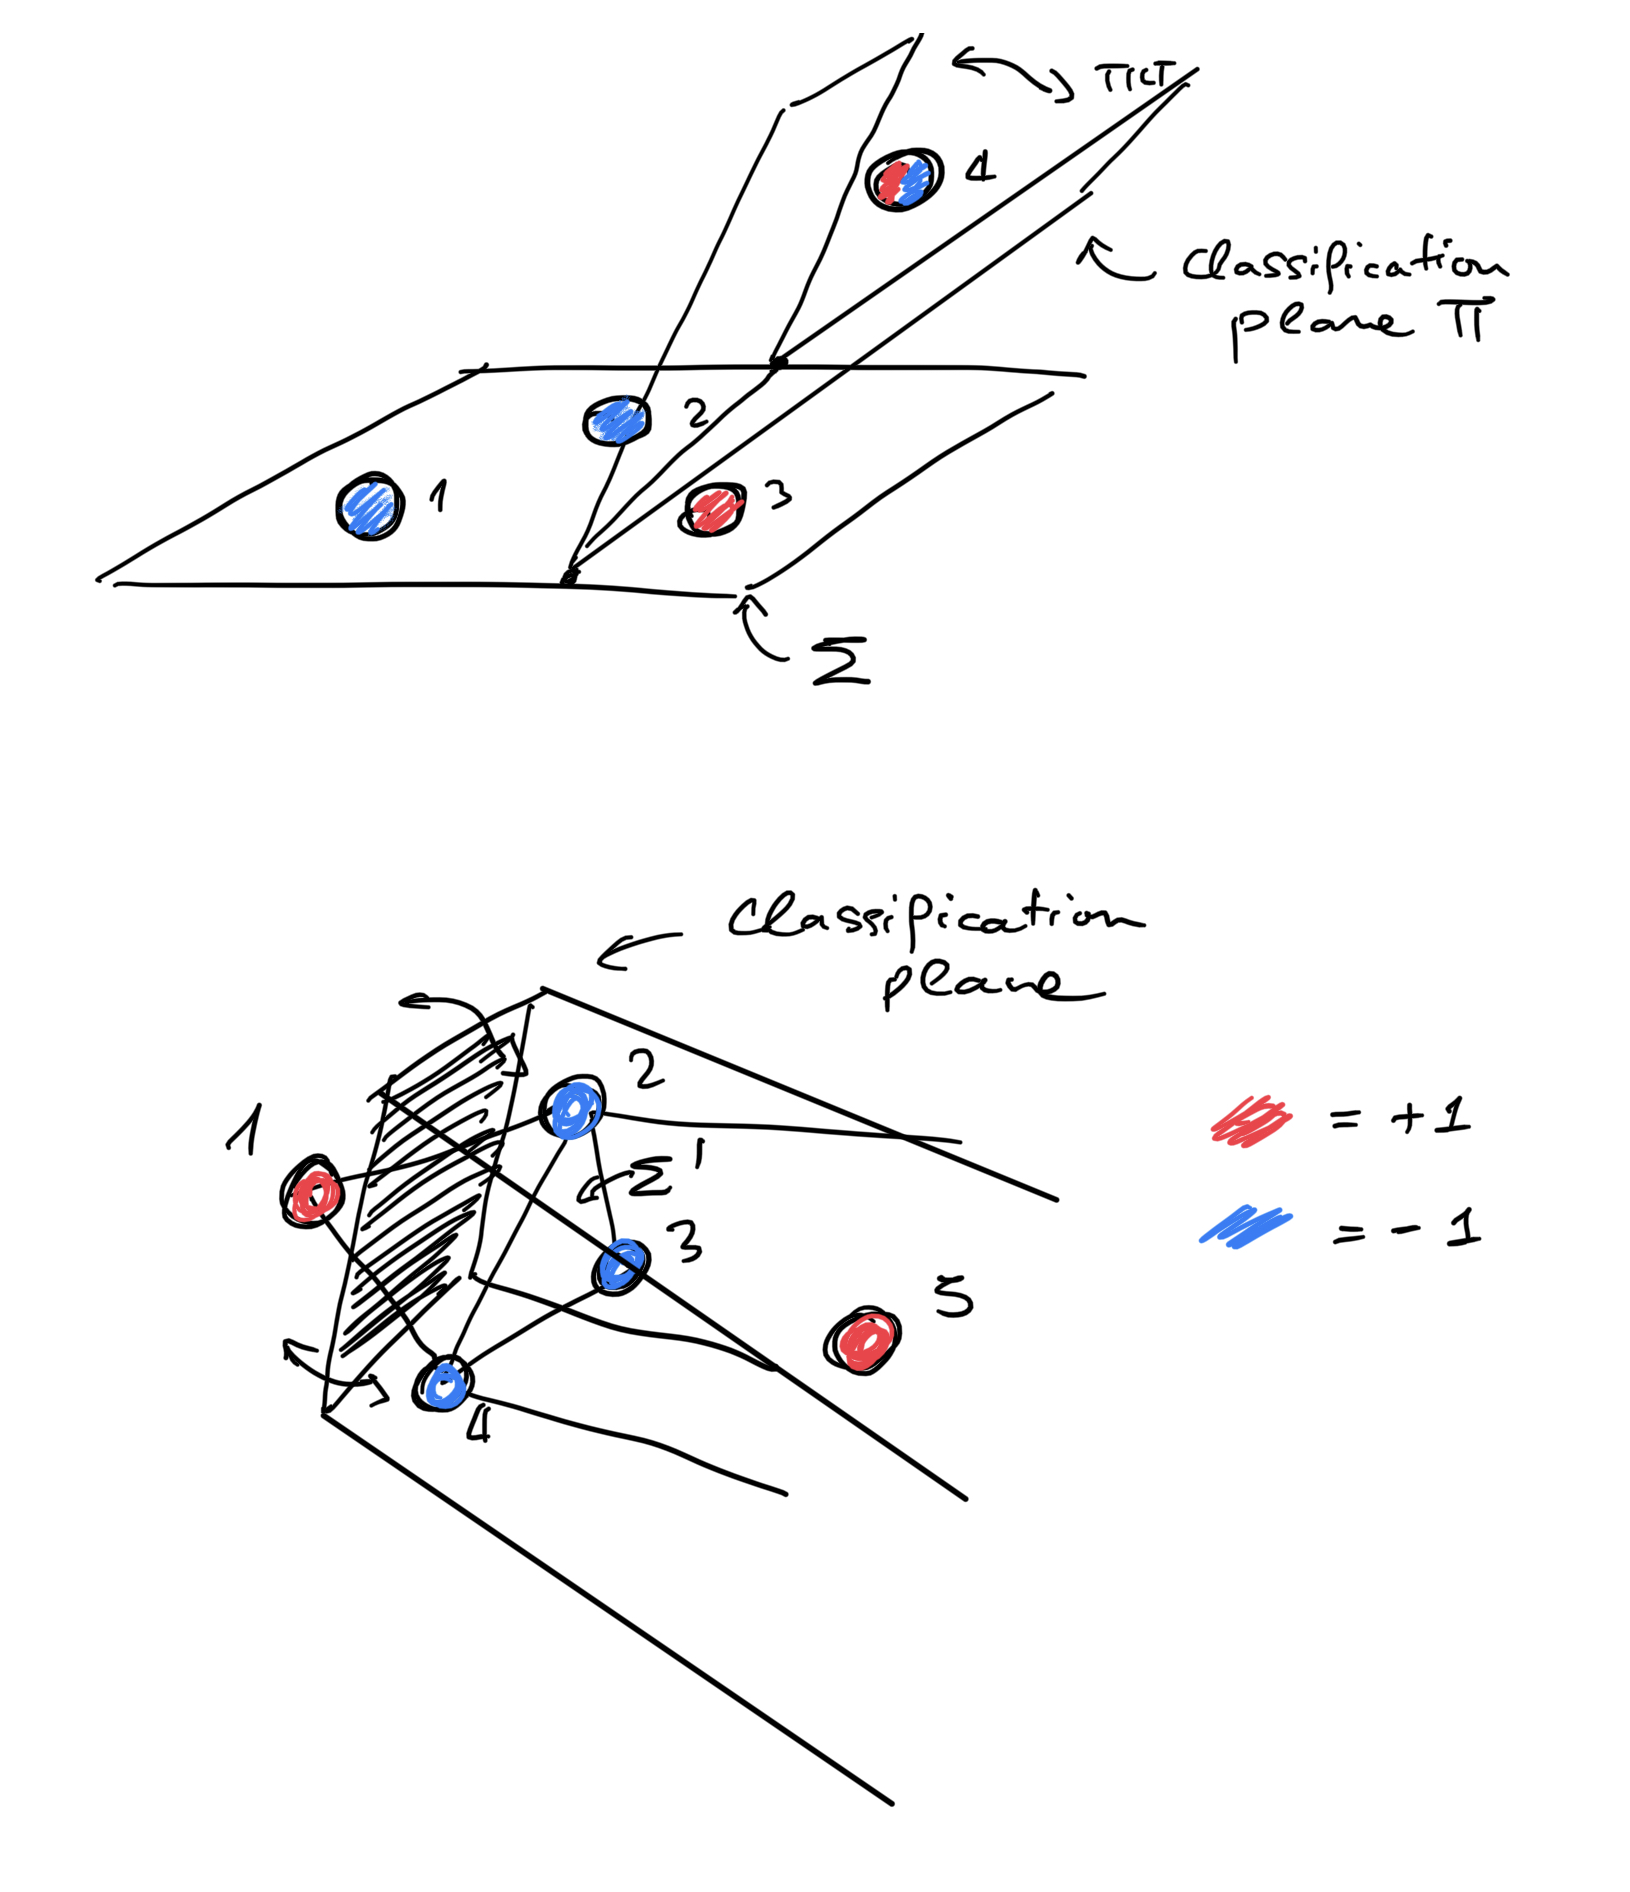
\includegraphics[scale=0.8]{Pset 3/IMG_0163.jpg}
    \caption{3D Perceptron and its break point}
    \label{fig:my_label}
\end{figure}
        
    \hypertarget{problem-5}{%
\section{Problem 5}\label{problem-5}}

\hypertarget{answer-b-iiiv}{%
\subsection{Answer: {[}b{]} i,ii,v}\label{answer-b-iiiv}}

\hypertarget{derivation}{%
\subsection{Derivation:}\label{derivation}}

A growth function \(m_{\mathcal{H}}(N)\) is well defined if one of the
two following conditions are satisfied:

\begin{itemize}
\tightlist
\item
  \(m_{\mathcal{H}}(N)= 2^N\) for any N, or
\item
  \(m_{\mathcal{H}}(N)\) is a polynomial function of N such that
  \(m_{\mathcal{H}}(N)\le 2^N\) for any \(N\).
\end{itemize}

In the following, we verify the proposed functions.

\begin{itemize}
\item
  \begin{enumerate}
  \def\labelenumi{\roman{enumi})}
  \tightlist
  \item
    \(f_1(N)=1+N \le 2^N\) OK!
  \end{enumerate}
\item
  \begin{enumerate}
  \def\labelenumi{\roman{enumi})}
  \setcounter{enumi}{1}
  \tightlist
  \item
    \(f_2(N)=1+N+{N\choose 2}=1+N+\frac{N!}{2!N-2!}=1+N+\frac{N!}{2!N-2!}=1+N+\frac{N(N-1)}{2}=1+\frac{N(N+1)}{2}\le 2^N\)
    OK!
  \end{enumerate}
\item
  \begin{enumerate}
  \def\labelenumi{\roman{enumi})}
  \setcounter{enumi}{2}
  \tightlist
  \item
    \(f_3(N)=\sum^{[\sqrt{N}]}_{i=1} {N\choose i} \ge \sum^{[\sqrt{N}]}_{i=0}{[\sqrt{N}]\choose i}-1=2^{[\sqrt{N}]}-1\).
    Hence, \(f_3(N)\) is greater than a non-polynomial function in N,
    although smaller than \(2^N\) for \(N\ge 1\). KO!
  \end{enumerate}
\item
  \begin{enumerate}
  \def\labelenumi{\roman{enumi})}
  \setcounter{enumi}{3}
  \tightlist
  \item
    \(f_4(N)=2^{[N/2]}\). Again, it is a non-polynomial function smaller
    than \(2^N\) for \(N\ge 1\). KO!
  \end{enumerate}
\item
  \begin{enumerate}
  \def\labelenumi{\alph{enumi})}
  \setcounter{enumi}{21}
  \tightlist
  \item
    \(f_5(N)=2^{N}\). Trivially, this is a valid growth function. OK!
  \end{enumerate}
\end{itemize}

    \hypertarget{problem-6}{%
\section{Problem 6}\label{problem-6}}

\hypertarget{answer-c-5}{%
\subsection{Answer: {[}c{]} 5}\label{answer-c-5}}

\hypertarget{derivation}{%
\subsection{Derivation:}\label{derivation}}

2-intervals hypothesis set can shatter completely a data set of four
points: this is because two intervals are able to reproduce all the
dichotomies for which the classification value of adjacent points
doesn't flip more than three times.

With 5 points we can easily conceive a dichotomy which is not reproduced
by the 2-intervals hypothesis set, in which the classification values
flip four times between adjacent points, e.g. \(\{+1,-1,+1,-1,+1\}\).
Therefore, the break point for the 2-intervals hypothesis set is 5.

    \hypertarget{problem-7}{%
\section{Problem 7}\label{problem-7}}

\hypertarget{answer-c-n1choose4n1choose21}{%
\subsection{\texorpdfstring{Answer: {[}c{]}
\({N+1\choose4}+{N+1\choose2}+1\)}{Answer: {[}c{]} \{N+1\textbackslash{}choose4\}+\{N+1\textbackslash{}choose2\}+1}}\label{answer-c-n1choose4n1choose21}}

\hypertarget{derivation}{%
\subsection{Derivation:}\label{derivation}}

In the following, we will prove the expression for the growth function
for the most generic \(M-\)intervals hypothesis set. We notice that
given \(N\) points, the line is split by the points into \(N+1\)
different regions. The dichotomy is fixed once we decide by which \(2M\)
regions contain the end values of the \(M\) intervals. If all the ends
of all the intervals do not overlap, there are \(N+1\choose2M\) possible
different dichotomies. If any two intervals are overlapped (i.e.~two of
their ends happens to be in the same region), they count as one, then
the number of possible choices reduces to \(N+1\choose2(M-1)\). This
recursively until we get the trivial hypothesis where both of the ends
of all the intervals collapse in the same region. In formulae:

\[
\label{growthfunc}
m_{\mathcal{H}(M)}(N)=\sum^M_{k=0} {N+1\choose2 k}\,.
\]

For \(M=2\) case, we get:

\[
m_{\mathcal{H}(2)}(N)=\sum^2_{k=0} {N+1\choose2 k}={N+1\choose4}+{N+1\choose2}+1\,.
\]

    \hypertarget{problem-8}{%
\section{Problem 8}\label{problem-8}}

\hypertarget{answer-d-2m1}{%
\subsection{\texorpdfstring{Answer: {[}d{]}
\(2M+1\)}{Answer: {[}d{]} 2M+1}}\label{answer-d-2m1}}

\hypertarget{derivation}{%
\subsection{Derivation:}\label{derivation}}

Generalizing the result of Problem 6, we notice that for the
\(M-\)intervals model, we need at least \(M+1\) flips of classification
value between adjacent points to reproduce a dichotomy that cannot be
generated by the model. To do that, we need at least \(N=2(M+1)-1\)
points, since the last point can be classified as the first. Therefore,
\(k=2M+1\). We can explicitly verify this result by studying the growth
function defined above in Eq.\(\,\eqref{growthfunc}\) behavior as a
function of \(M\).

    \begin{tcolorbox}[breakable, size=fbox, boxrule=1pt, pad at break*=1mm,colback=cellbackground, colframe=cellborder]
\prompt{In}{incolor}{6}{\boxspacing}
\begin{Verbatim}[commandchars=\\\{\}]
\PY{k+kn}{import} \PY{n+nn}{scipy}\PY{n+nn}{.}\PY{n+nn}{special}
\PY{k+kn}{import} \PY{n+nn}{matplotlib}\PY{n+nn}{.}\PY{n+nn}{pyplot} \PY{k}{as} \PY{n+nn}{plt}

\PY{k}{def} \PY{n+nf}{growth\PYZus{}func}\PY{p}{(}\PY{n}{M}\PY{p}{,}\PY{n}{N}\PY{p}{)}\PY{p}{:}
    \PY{n}{m}\PY{o}{=}\PY{l+m+mi}{0}
    \PY{k}{for} \PY{n}{i} \PY{o+ow}{in} \PY{n+nb}{range}\PY{p}{(}\PY{n}{M}\PY{o}{+}\PY{l+m+mi}{1}\PY{p}{)}\PY{p}{:}
       \PY{n}{m}\PY{o}{+}\PY{o}{=}\PY{n}{scipy}\PY{o}{.}\PY{n}{special}\PY{o}{.}\PY{n}{binom}\PY{p}{(}\PY{n}{N}\PY{o}{+}\PY{l+m+mi}{1}\PY{p}{,}\PY{l+m+mi}{2}\PY{o}{*}\PY{n}{i}\PY{p}{)}
    \PY{k}{return} \PY{n}{np}\PY{o}{.}\PY{n}{int}\PY{p}{(}\PY{n}{m}\PY{p}{)}

\PY{k}{def} \PY{n+nf}{break\PYZus{}point}\PY{p}{(}\PY{n}{growth\PYZus{}func}\PY{p}{,} \PY{n}{M}\PY{p}{)}\PY{p}{:}
    \PY{n}{brk\PYZus{}pt}\PY{o}{=}\PY{k+kc}{False}
    \PY{n}{N}\PY{o}{=}\PY{l+m+mi}{0}
    \PY{k}{while}\PY{p}{(}\PY{n}{brk\PYZus{}pt}\PY{o}{==}\PY{k+kc}{False}\PY{p}{)}\PY{p}{:}
        \PY{n}{brk\PYZus{}pt}\PY{o}{=}\PY{p}{(}\PY{n}{growth\PYZus{}func}\PY{p}{(}\PY{n}{M}\PY{p}{,}\PY{n}{N}\PY{p}{)}\PY{o}{\PYZlt{}}\PY{l+m+mi}{2}\PY{o}{*}\PY{o}{*}\PY{n}{N}\PY{p}{)}
        \PY{n}{N}\PY{o}{+}\PY{o}{=}\PY{l+m+mi}{1}
    \PY{k}{return} \PY{n}{N}\PY{o}{\PYZhy{}}\PY{l+m+mi}{1}
        
\PY{n}{xrange}\PY{o}{=}\PY{n}{np}\PY{o}{.}\PY{n}{array}\PY{p}{(}\PY{n+nb}{range}\PY{p}{(}\PY{l+m+mi}{20}\PY{p}{)}\PY{p}{)}
\PY{n}{bpts}\PY{o}{=}\PY{p}{[}\PY{n}{break\PYZus{}point}\PY{p}{(}\PY{n}{growth\PYZus{}func}\PY{p}{,} \PY{n}{xrange}\PY{p}{[}\PY{n}{i}\PY{p}{]}\PY{p}{)} \PY{k}{for} \PY{n}{i} \PY{o+ow}{in} \PY{n}{xrange}\PY{p}{]}
\PY{n}{plt}\PY{o}{.}\PY{n}{plot}\PY{p}{(}\PY{n}{xrange}\PY{p}{,}\PY{l+m+mi}{2}\PY{o}{*}\PY{n}{xrange}\PY{o}{+}\PY{l+m+mi}{1}\PY{p}{,} \PY{n}{label}\PY{o}{=}\PY{l+s+s2}{\PYZdq{}}\PY{l+s+s2}{b(M)=2M+1}\PY{l+s+s2}{\PYZdq{}}\PY{p}{,} \PY{n}{color}\PY{o}{=}\PY{l+s+s1}{\PYZsq{}}\PY{l+s+s1}{red}\PY{l+s+s1}{\PYZsq{}}\PY{p}{)}
\PY{n}{plt}\PY{o}{.}\PY{n}{scatter}\PY{p}{(}\PY{n}{xrange}\PY{p}{,} \PY{n}{bpts}\PY{p}{,}\PY{n}{label}\PY{o}{=}\PY{l+s+s1}{\PYZsq{}}\PY{l+s+s1}{break points}\PY{l+s+s1}{\PYZsq{}}\PY{p}{)}
\PY{n}{plt}\PY{o}{.}\PY{n}{legend}\PY{p}{(}\PY{p}{)}
\PY{n}{plt}\PY{o}{.}\PY{n}{show}\PY{p}{(}\PY{p}{)}
\end{Verbatim}
\end{tcolorbox}

    \begin{center}
    \adjustimage{max size={0.9\linewidth}{0.9\paperheight}}{output_9_0.png}
    \end{center}
    { \hspace*{\fill} \\}
    
    \hypertarget{problem-9}{%
\section{Problem 9}\label{problem-9}}

\hypertarget{answer-d-7}{%
\subsection{Answer: {[}d{]} 7}\label{answer-d-7}}

\hypertarget{derivation}{%
\subsection{Derivation:}\label{derivation}}

In this problem, we are asked to compute the largest number of points on
the plane that can be shattered by a triangle hypothesis set, also
knowns as its VC dimension \(d_{VC}\). We can proceed more generally and
ask what is the VC dimension \(d_{VC}(n)\) of a generic convex \(n-\)gon
classification model on a plane. We can easily prove by simple arguments
that \(d_{VC}(n)=2n+1\) in two steps:

\begin{itemize}
\tightlist
\item
  \(d_{VC}(n)\ge2n+1\)
\end{itemize}

We choose to put our \(2n+1\) points on a circle. The only delicate
dichotomies to be checked are the ones with \(n\) or \(n+1\) points that
must be inside the poligon. In the first case, we will choose the \(n\)
points as the vertices of the polygon while in the other case we will
take the outer \(n\) points as tangent to the sides of the polygon. As
an illustration, the triangle case is shown in the following. Therefore,
we showed that a convex \(n-\)gon can shatter \(2n+1\) points on a
plane. Hence, its VC dimension has to be greater and equal than
\(2n+1\).

 \begin{figure}
    \centering
    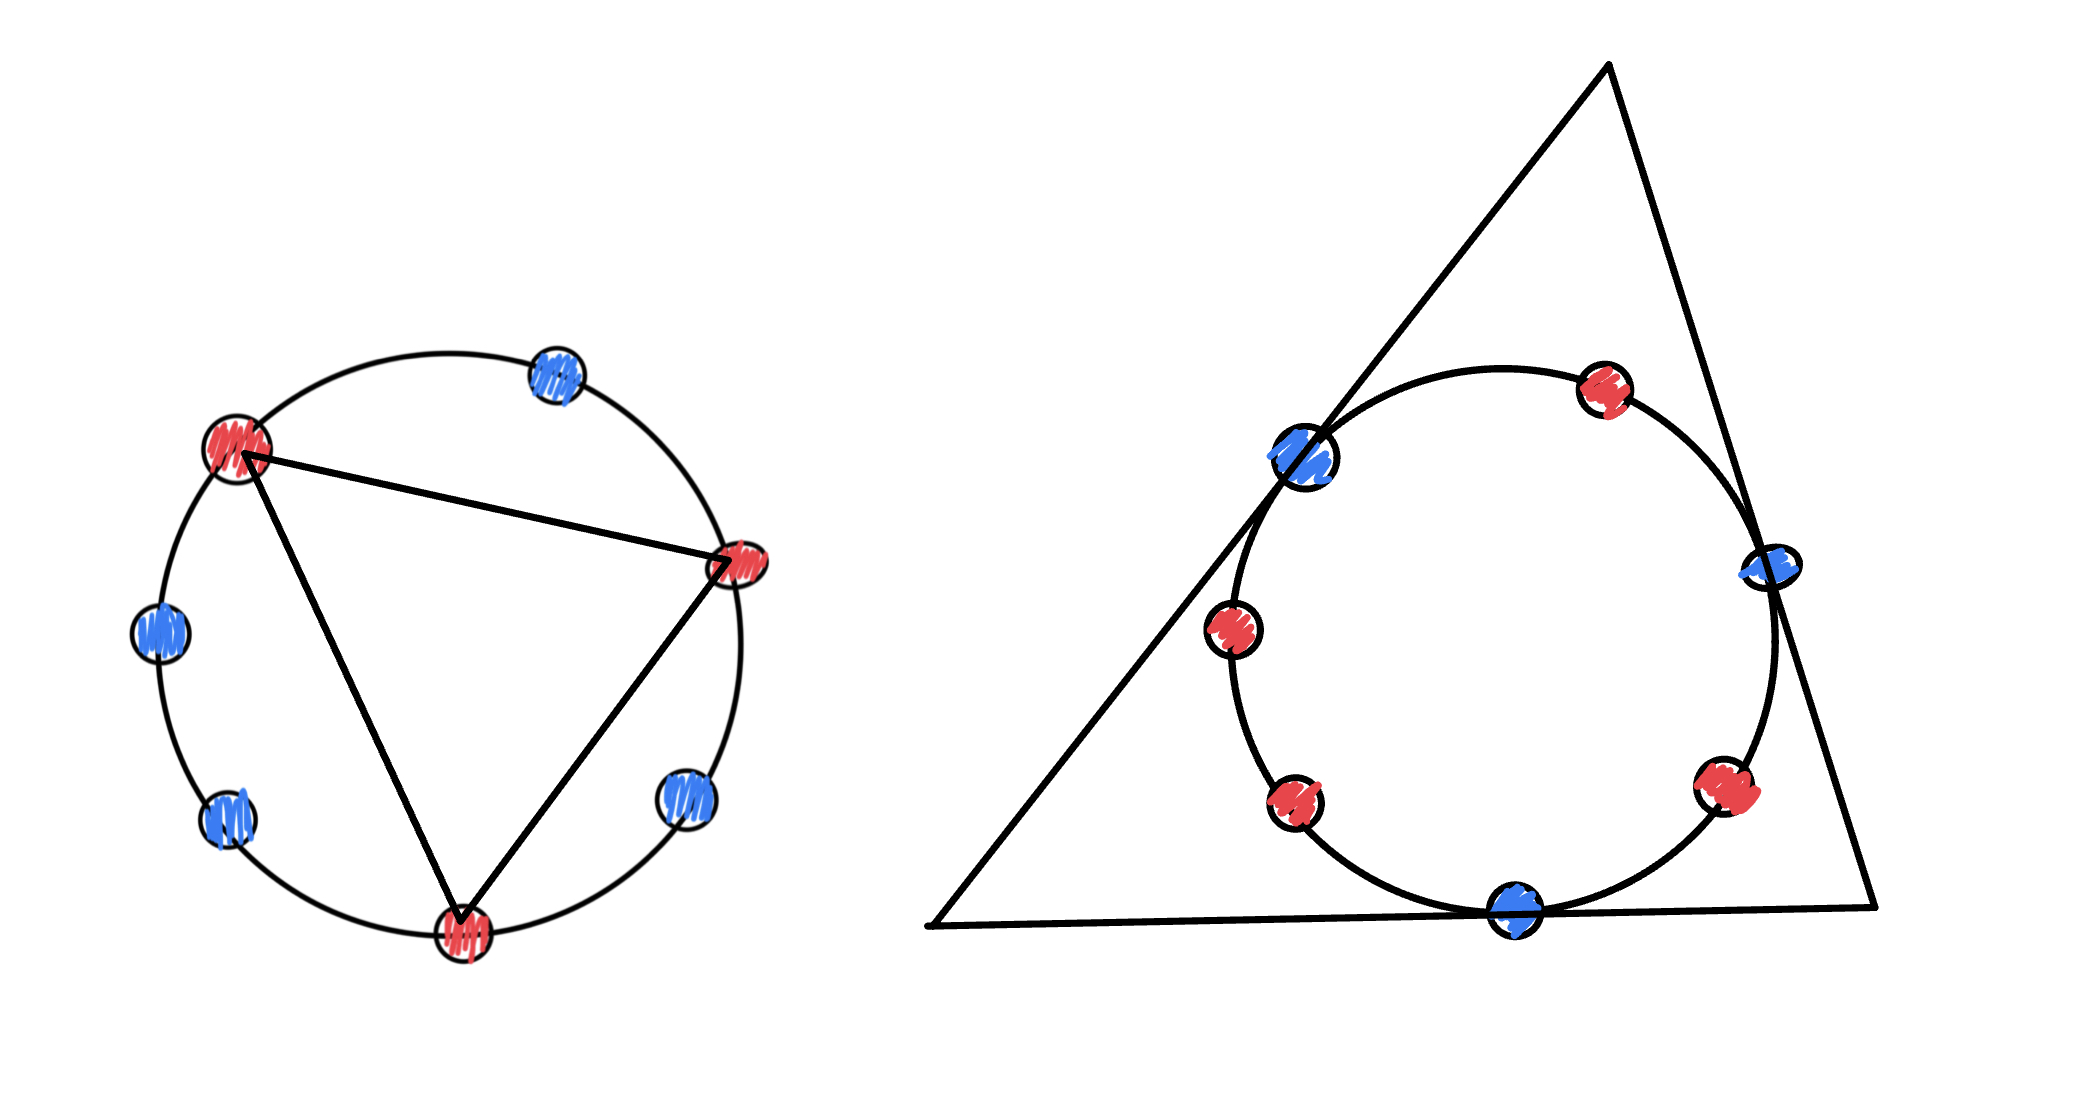
\includegraphics[scale=0.8]{Pset 3/IMG_0164.jpg}
    \caption{Triangle shattering 7 points on a plane: two interesting configurations.}
    \label{fig:my_label}
\end{figure}
        
    \begin{itemize}
\tightlist
\item
  \(d_{VC}(n)\le 2n+1\)
\end{itemize}

In this case, we should be more careful and not assume a specific
configuration for \(2n+2\) points. There are two possible cases: either
all the \(2n+2\) points lie on a convex polygon \(\mathcal{P}\) or there
is at least one point inside the polygon described by the other ones. We
can show now that there are two specific labeling that cannot be
reproduced by the \(n-\)gon in both cases.

\begin{itemize}
\item
  First case: all the points lie on a convex polygon. If we alternate
  their labeling, we will need at least \(n+1\) lines to separate the
  patterns since the convexity of \(\mathcal{P}\) doesn't allow to
  points to be separated by an internal line.
\item
  Second case: there is (at least) one point in the convex hull
  \(\mathcal{P}^\prime\) of the other ones. In this case, the labeling
  that cannot be reproduced is when all points in the outer polygon are
  classified inside the \(n-\)gon and the point(s) inside is not.
  Clearly, any classification \(n-\)gon we may use completely includes
  \(\mathcal{P}^\prime\), forcing its labeling to be the same as the
  other ones.
\end{itemize}

An illustration of the two cases for the triangle classifier with \(8\)
points is in the following.

\begin{figure}
    \centering
    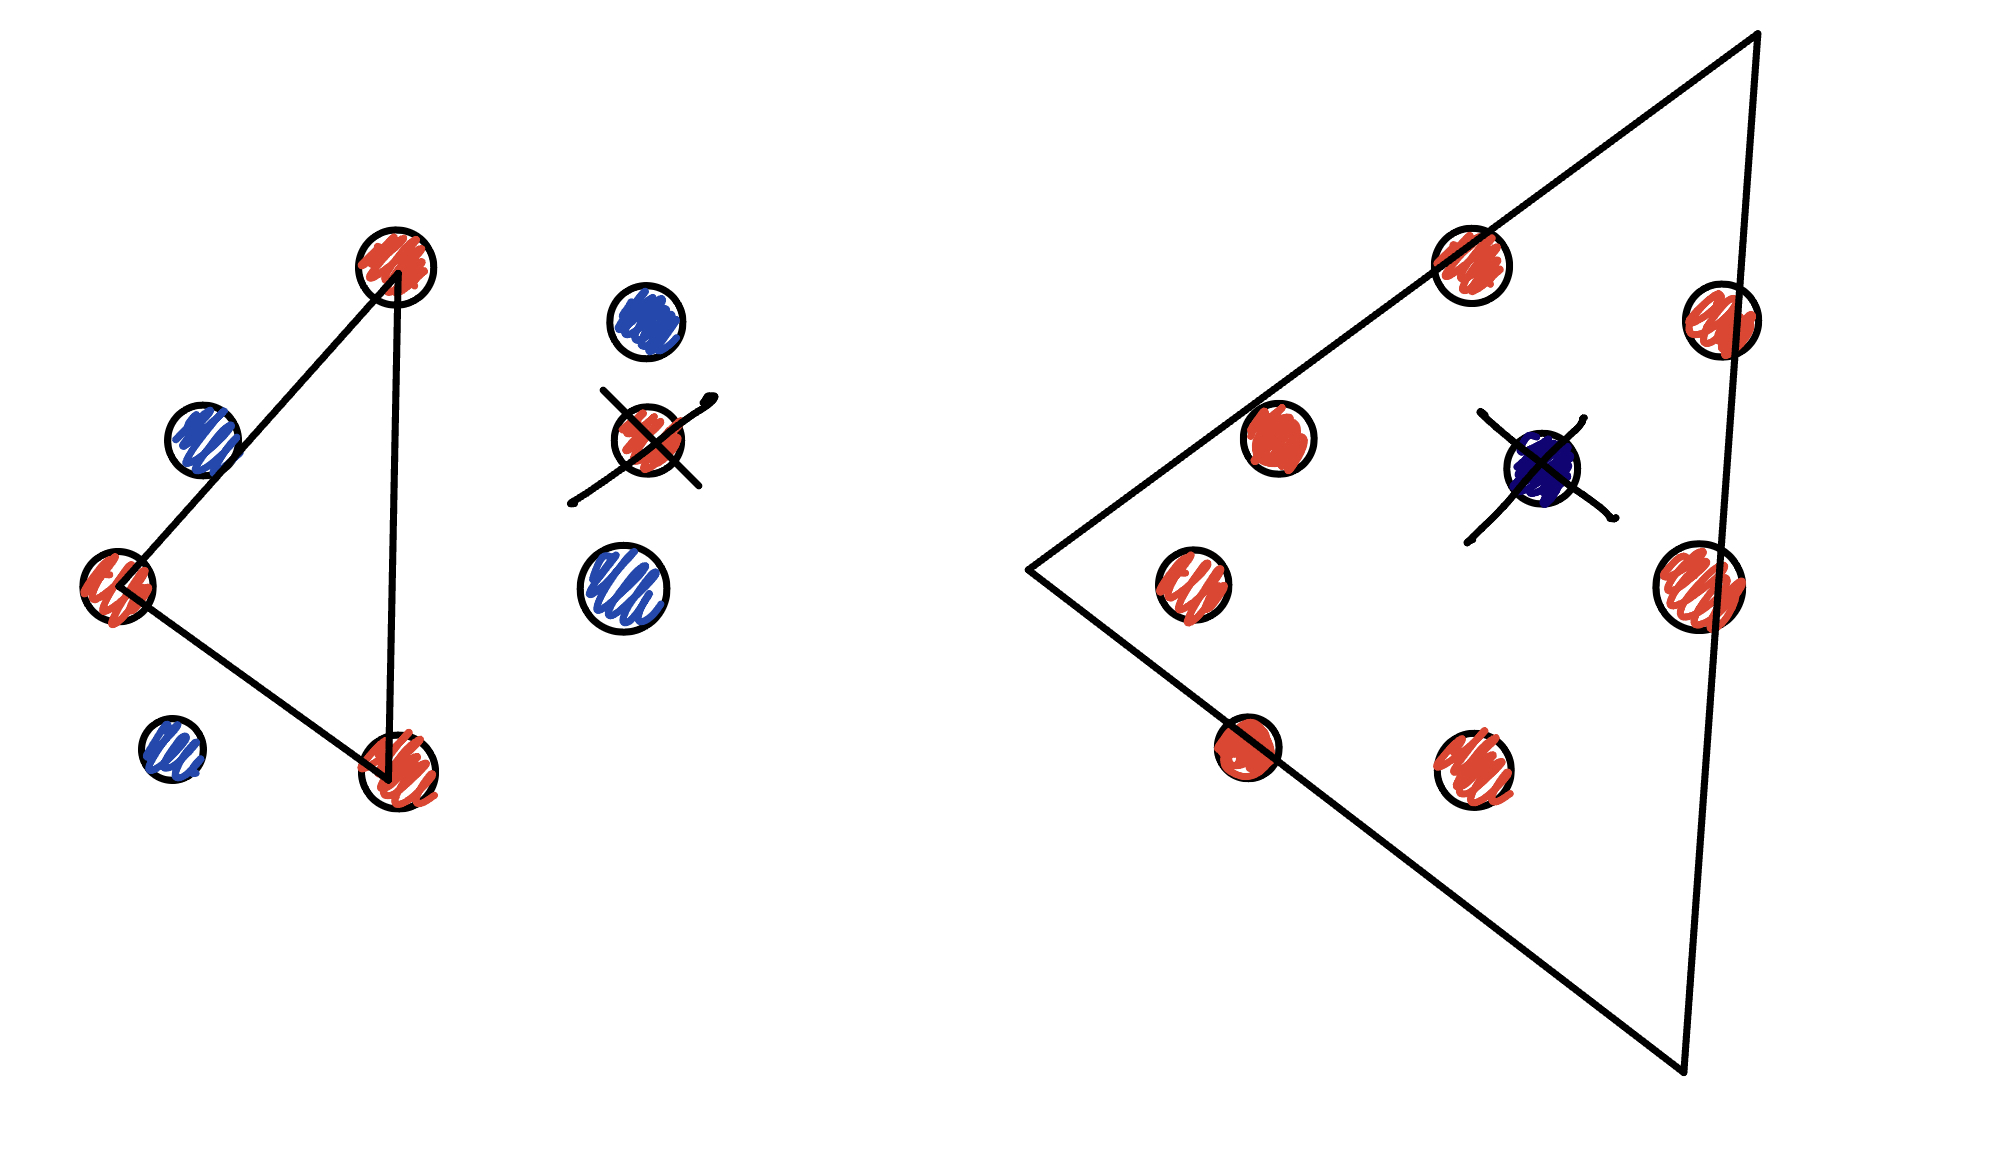
\includegraphics[scale=0.8]{Pset 3/IMG_0165.jpg}
    \caption{Break point for the triangle classifier.}
    \label{fig:my_label}
\end{figure}

\pagebreak

    \hypertarget{problem-10}{%
\section{Problem 10}\label{problem-10}}

\hypertarget{answer-b-n1choose21}{%
\subsection{\texorpdfstring{Answer: {[}b{]}
\({N+1\choose2}+1\)}{Answer: {[}b{]} \{N+1\textbackslash{}choose2\}+1}}\label{answer-b-n1choose21}}

\hypertarget{derivation}{%
\subsection{Derivation:}\label{derivation}}

If we act on the data points we have through a non-linear
transformation, parametrizing the data points as a function of their
distance squared form the origin \(\rho^2=x_1^2+x_2^2\), the
classification model of concentric circles reduces to the
1-(positive)interval model we explored above. Hence, the growth function
will be the same, i.e.

\[
m_{\mathcal{H}(1)}(N)=\sum^1_{k=0} {N+1\choose2 k}={N+1\choose2}+1\,.
\]


    % Add a bibliography block to the postdoc
    
    
    
\end{document}
